\documentclass[spanish, a4paper, 12pt, final, slideColor, nototal, colorBG, pdf, noaccumulate, darkblue] {beamer}
\usepackage[spanish]{babel}
\usepackage[utf8]{inputenc}
\usepackage{amsmath}
\usepackage{amssymb}
\usepackage{amsfonts}
\usepackage{latexsym}
\usepackage{mathtools}
\usepackage{anysize}
%\marginsize{2cm}{2cm}{2cm}{3cm}
\usepackage{soul}
\usepackage{mathtools}
\DeclarePairedDelimiter{\ceil}{\lceil}{\rceil}
\newcommand\eqdef{\stackrel{\mathclap{\mbox{\tiny{def}}}}{=}}
\newcommand\eqac{\stackrel{\mathclap{\mbox{*}}}{=}}

\usepackage{graphicx}
\usepackage{hyperref}
\usepackage{float}
\usepackage{verbatim}
\usepackage{caption}
\captionsetup{font=scriptsize,labelfont=scriptsize}
\DeclareGraphicsExtensions{.pdf,.png,.jpg}

\usetheme{Madrid}

\title{TOR}
\subtitle{Introducción a Onion Routing y Hidden Services}
\author{Marco Antonio Garrido Rojo\thanks{\url{https://github.com/MaSteve/TOR}}}
\date{4 de diciembre de 2017}

\begin{document}
\maketitle
\begin{frame}
    \frametitle{¿Qué es TOR?}
    \begin{itemize}
    \item Tor (acrónimo de The Onion Router) es un software para establecer comunicaciones anónimas a través de Internet.
    \item Su objetivo es proporcionar a sus usuarios un modo de comunicación confidencial.
    \item Basado en el principio de ``onion routing'' desarrollado por el gobierno de Estados Unidos en los 90.
    \item Más información sobre el proyecto: \url{torproject.org}
    \end{itemize}
\end{frame}
\begin{frame}
    \frametitle{¿Qué vamos a aprender hoy?}
    \begin{itemize}
    \item Fundamentos del ``onion routing''.
    \item Fundamentos de los Hidden Services.
    \item {\bf No} vamos a hablar de Deep Web.
    \end{itemize}
\end{frame}
\begin{frame}
    \frametitle{Criptografía: breve repaso}
    \begin{itemize}
    \item Tor no obliga a encriptar la comunicación. Canal anónimo no es lo mismo que mensaje oculto.
    \item Necesita hacer uso de la criptografía para garantizar el anonimato.
    \item Diffie-Hellman + Criptografía de dos claves (clave pública).
    \end{itemize}
\end{frame}
\begin{frame}
    \frametitle{Criptografía: breve repaso}
    \begin{itemize}
    \item Diffie-Hellman es un método de establecimiento seguro de claves.
    \item A partir de una información conocida por todos (incluso por un man in the middle) se comparte un secreto conocido solo por los dos extremos.
    \end{itemize}
    \begin{figure}[!ht]
      \centering
      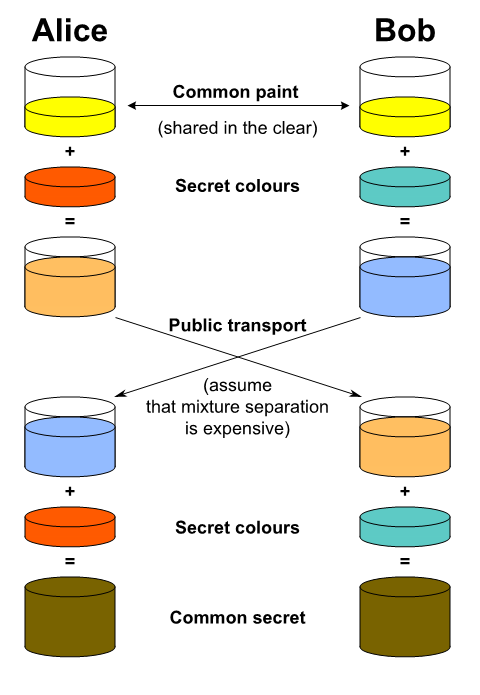
\includegraphics[scale=0.25]{Diffie-Hellman-Wikipedia.png}
      \caption{Illustration of the idea behind Diffie-Hellman key Exchange (Wikipedia)}
    \end{figure}
\end{frame}
\begin{frame}
    \frametitle{Criptografía: breve repaso}
    \begin{itemize}
    \item La criptografía de clave pública garantiza una comunicación unidireccional segura.
    \item El emisor puede encriptar mensajes usando la clave pública. Solo el receptor puede descifrar el mensaje con la clave privada.
    \end{itemize}
    \begin{figure}[!ht]
      \centering
      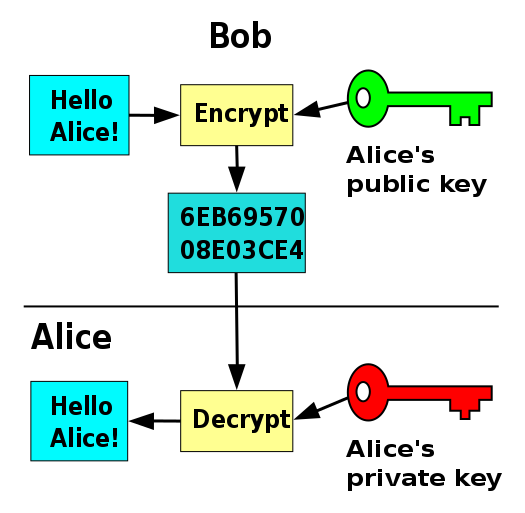
\includegraphics[scale=0.25]{Public-key-Wikipedia.png}
      \caption{Illustration of Public-key cryptography (Wikipedia)}
    \end{figure}
\end{frame}
\begin{frame}
    \frametitle{Criptografía: breve repaso}
    \begin{figure}[!ht]
      \centering
      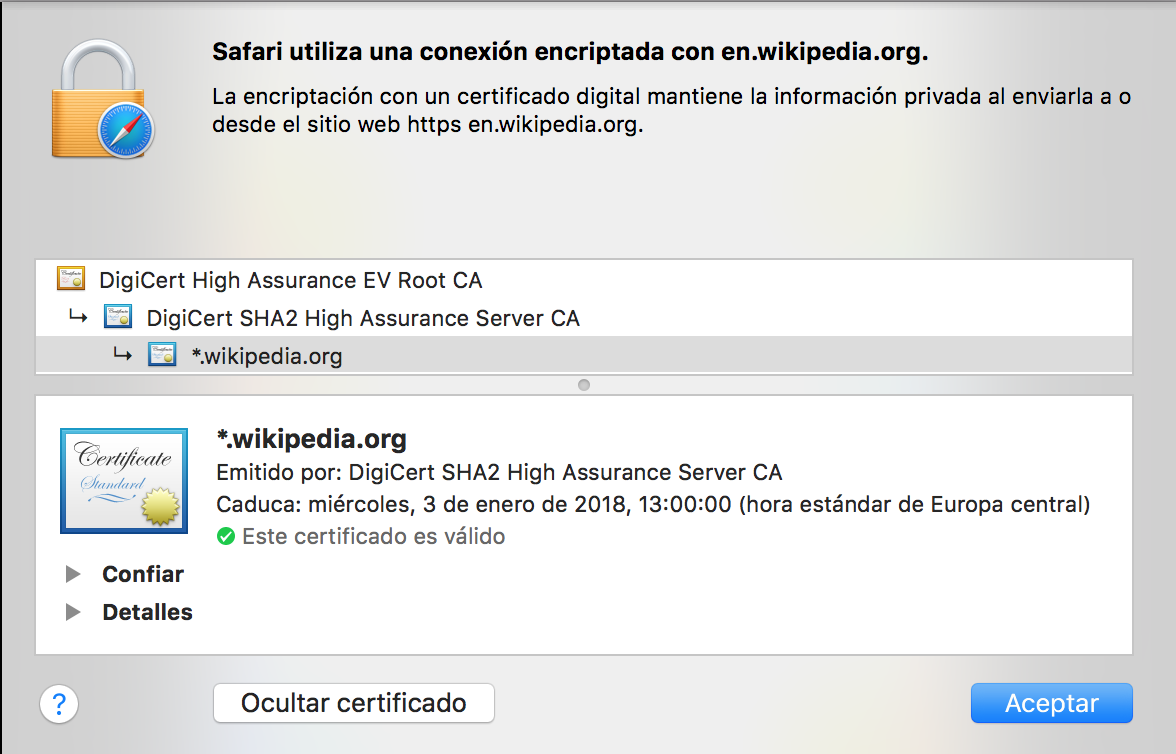
\includegraphics[scale=0.5]{Certificado.png}
      %\caption{Certificado (Wikipedia)}
    \end{figure}
\end{frame}
\begin{frame}
    \frametitle{¿Qué problema queremos resolver?}
    \begin{itemize}
    \item Alice (cliente) quiere hablar con Bob (servidor) sin que nadie sepa que ambos están hablando.
    \item No puede haber una conexión directa (man in the middle).
    \item Un VPN o un proxy actúan de puente pero conocen los extremos (hay que confiar).
    \item Una red de proxies parece ser la solución (con cuidado). Hay que garantizar que el usuario es completamente anónimo (nodos públicos y conocidos).
    \item Cada nodo solo puede conocer lo justo y necesario.
    \item ``Onion routing'' es la solución.
    \end{itemize}
\end{frame}
\begin{frame}
    \frametitle{¿Qué problemas tiene?}
    \begin{itemize}
    \item Comunicación no cifrada al final de la cadena (HTTP).
    \item Javascript puede obtener datos del cliente (MAC + IP).
    \item DNS sin Tor (fin de la magia).
    \item Escuchar mensajes al principio y al final de la cadena + Estadística.
    \end{itemize}
\end{frame}
\begin{frame}
    \frametitle{¿Qué son los Hidden Services?}
    \begin{itemize}
    \item ¿Qué ocurre si soy un servidor?
    \item Alice y Bob quieren permanecer ocultos en sus casas y comunicarse al mismo tiempo.
    \item Los Hidden Services solucionan este problema.
    \item ¿Cómo? ``Onion routing'' + Tabla hash de descriptores distribuida.
    \end{itemize}
\end{frame}
\begin{frame}
    \frametitle{Preguntas}
    \center ¿Preguntas? No os cortéis, es vuestro momento.
\end{frame}
\end{document}
